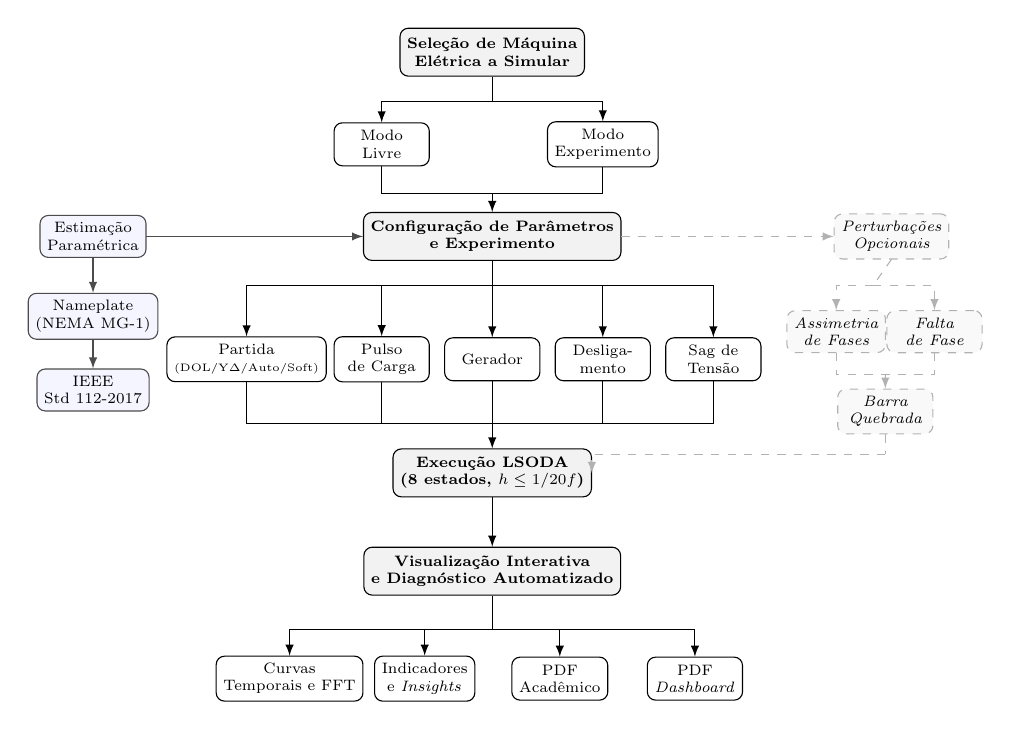
\begin{tikzpicture}[
    scale=0.78, transform shape,
    % Nós comuns
    no/.style={
        draw, rounded corners=3pt, fill=white,
        font=\scriptsize, minimum width=1.55cm,
        minimum height=0.7cm, align=center
    },
    % Nós de destaque
    nodest/.style={
        draw, rounded corners=3pt, fill=gray!10,
        font=\scriptsize\bfseries, minimum width=2.6cm,
        minimum height=0.78cm, align=center
    },
    % Nós opcionais (perturbações)
    noopt/.style={
        draw=gray!60, dashed, rounded corners=3pt, fill=gray!5,
        font=\scriptsize\itshape, minimum width=1.55cm,
        minimum height=0.65cm, align=center
    },
    % Nós laterais de estimação
    noest/.style={
        draw=black!70, rounded corners=3pt, fill=blue!4,
        font=\scriptsize, minimum width=1.7cm,
        minimum height=0.65cm, align=center
    },
    linha/.style={draw, thin, -latex},
    lopt/.style={draw=gray!60, thin, dashed, -latex},
    lest/.style={draw=black!70, thin, -latex}
]

% ---- NÍVEL 0: RAIZ ----
\node[nodest] (raiz) at (0, 0) {Seleção de Máquina\\Elétrica a Simular};

% ---- NÍVEL 1: MODOS ----
\node[no] (m_livre) at (-1.8, -1.5) {Modo\\Livre};
\node[no] (m_exp)   at ( 1.8, -1.5) {Modo\\Experimento};

\coordinate (bif_modo) at (0, -0.8);
\draw[thin]  (raiz.south)   -- (bif_modo);
\draw[linha] (bif_modo) -| (m_livre.north);
\draw[linha] (bif_modo) -| (m_exp.north);

% ---- NÍVEL 2: CONFIGURAÇÃO ----
\node[nodest] (config) at (0, -3.0) {Configuração de Parâmetros\\e Experimento};

\coordinate (merge_modo) at (0, -2.3);
\draw[thin]  (m_livre.south) |- (merge_modo);
\draw[thin]  (m_exp.south)   |- (merge_modo);
\draw[linha] (merge_modo) -- (config.north);

% ---- ESTIMAÇÃO PARAMÉTRICA (lateral esquerda) ----
\node[noest] (est_root) at (-6.5, -3.0) {Estimação\\Paramétrica};
\node[noest] (est_np)   at (-6.5, -4.3) {Nameplate\\(NEMA MG-1)};
\node[noest] (est_iee)  at (-6.5, -5.5) {IEEE\\Std 112-2017};

\draw[lest] (est_root.south) -- (est_np.north);
\draw[lest] (est_np.south)   -- (est_iee.north);
\draw[lest] (est_root.east)  -- (config.west);

% ---- PERTURBAÇÕES OPCIONAIS (lateral direita) ----
\node[noopt] (perturb) at (6.5, -3.0)  {Perturbações\\Opcionais};
\node[noopt] (p_assim) at (5.6, -4.55) {Assimetria\\de Fases};
\node[noopt] (p_falta) at (7.2, -4.55) {Falta\\de Fase};
\node[noopt] (p_bb)    at (6.4, -5.85) {Barra\\Quebrada};

\draw[lopt] (config.east) -- (perturb.west);

% Bifurcação das perturbações alinhada ao centro do nó pai
\coordinate (bif_p) at (6.2, -3.8);
\draw[draw=gray!60, thin, dashed] (perturb.south) -- (bif_p);
\draw[lopt] (bif_p) -| (p_assim.north);
\draw[lopt] (bif_p) -| (p_falta.north);

% Barra quebrada agregada na descida
\draw[draw=gray!60, thin, dashed] (p_assim.south) |- (6.4, -5.25);
\draw[draw=gray!60, thin, dashed] (p_falta.south) |- (6.4, -5.25);
\draw[lopt] (6.4, -5.25) -- (p_bb.north);

\coordinate (merge_p) at (6.4, -6.55);
\draw[draw=gray!60, thin, dashed] (p_bb.south) -- (merge_p);

% ---- NÍVEL 3: GRUPOS DE CENÁRIOS (5 grupos cobrindo 8 modos) ----
\node[no, minimum width=2.1cm] (g1) at (-4.0, -5.0) {Partida\\\tiny(DOL/Y$\Delta$/Auto/Soft)};
\node[no] (g2) at (-1.8, -5.0) {Pulso\\de Carga};
\node[no] (g3) at ( 0.0, -5.0) {Gerador};
\node[no] (g4) at ( 1.8, -5.0) {Desliga-\\mento};
\node[no] (g5) at ( 3.6, -5.0) {Sag de\\Tensão};

\coordinate (bif_e) at (0, -3.8);
\draw[thin]  (config.south) -- (bif_e);
\draw[linha] (bif_e) -| (g1.north);
\draw[linha] (bif_e) -| (g2.north);
\draw[linha] (bif_e) -- (g3.north);
\draw[linha] (bif_e) -| (g4.north);
\draw[linha] (bif_e) -| (g5.north);

% ---- NÍVEL 4: EXECUÇÃO ----
\node[nodest] (sim) at (0, -6.85) {Execução LSODA\\(8 estados, $h \leq 1/20f$)};

\coordinate (merge_e) at (0, -6.05);
\draw[thin]  (g1.south) |- (merge_e);
\draw[thin]  (g2.south) |- (merge_e);
\draw[thin]  (g3.south) |- (merge_e);
\draw[thin]  (g4.south) |- (merge_e);
\draw[thin]  (g5.south) |- (merge_e);
\draw[linha] (merge_e)  -- (sim.north);

% Conexão única vinda do bloco de perturbações
\draw[lopt] (merge_p) -| (sim.east);

% ---- NÍVEL 5: VISUALIZAÇÃO + DIAGNÓSTICO ----
\node[nodest] (vis) at (0, -8.45) {Visualização Interativa\\e Diagnóstico Automatizado};
\draw[linha] (sim.south) -- (vis.north);

% ---- NÍVEL 6: SAÍDAS ----
\node[no, minimum width=1.55cm] (a1) at (-3.3, -10.2) {Curvas\\Temporais e FFT};
\node[no, minimum width=1.55cm] (a2) at (-1.1, -10.2) {Indicadores\\e \emph{Insights}};
\node[no, minimum width=1.55cm] (a3) at ( 1.1, -10.2) {PDF\\Acadêmico};
\node[no, minimum width=1.55cm] (a4) at ( 3.3, -10.2) {PDF\\\emph{Dashboard}};

\coordinate (bif_a) at (0, -9.4);
\draw[thin]  (vis.south) -- (bif_a);
\draw[linha] (bif_a) -| (a1.north);
\draw[linha] (bif_a) -| (a2.north);
\draw[linha] (bif_a) -| (a3.north);
\draw[linha] (bif_a) -| (a4.north);

\end{tikzpicture}
